\documentclass[13pt,a4paper]{article}
\usepackage{a4wide,amssymb,epsfig,latexsym,multicol,array,hhline,fancyhdr}
\usepackage{amsmath}
\usepackage{amsfonts}
\usepackage{lastpage}
\usepackage[lined,boxed,commentsnumbered]{algorithm2e}
\usepackage{enumerate}
\usepackage{color}
\usepackage{graphicx}							% Standard graphics package
\usepackage{array}
\usepackage{tabularx, caption}
\usepackage{multirow}
\usepackage{multicol}
\usepackage{rotating}
\usepackage{graphics}
\usepackage{geometry}
\usepackage{setspace}
\usepackage{subfig}
\usepackage{epsfig}
\usepackage{tikz}
\usepackage[
   sorting=none, 
	backend=biber,
	style=alphabetic,
]{biblatex}
\addbibresource{reference.bib}
\usetikzlibrary{arrows,snakes,backgrounds}
\usepackage{hyperref}
\hypersetup{urlcolor=blue,linkcolor=black,citecolor=black,colorlinks=true} 
%\usepackage{pstcol} 								% PSTricks with the standard color package

\newtheorem{theorem}{{\bf Theorem}}
\newtheorem{property}{{\bf Property}}
\newtheorem{proposition}{{\bf Proposition}}
\newtheorem{corollary}[proposition]{{\bf Corollary}}
\newtheorem{lemma}[proposition]{{\bf Lemma}}

\AtBeginDocument{\renewcommand*\contentsname{Contents}}
\AtBeginDocument{\renewcommand*\refname{References}}
%\usepackage{fancyhdr}
\setlength{\headheight}{40pt}
\pagestyle{fancy}
\fancyhead{} % clear all header fields
\fancyhead[L]{
	\begin{tabular}{rl}
		\begin{picture}(25,15)(0,0)
			\put(0,-8){
\includegraphics[width=8mm, height=8mm]{hcmut.png}}
			%\put(0,-8){\epsfig{width=10mm,figure=hcmut.eps}}
		\end{picture}&
		%
\includegraphics[width=8mm, height=8mm]{hcmut.png} & %
		\begin{tabular}{l}
			\textbf{\bf \ttfamily Ho Chi Minh University of Technology}\\
			\textbf{\bf \ttfamily Faculty of Computer Science and Engineering}
		\end{tabular} 	
	\end{tabular}
}
\fancyhead[R]{
	\begin{tabular}{l}
		\tiny \bf \\
		\tiny \bf 
\end{tabular}  }
\fancyfoot{} % clear all footer fields
\fancyfoot[L]{\scriptsize \ttfamily Assignment Report for Operating systems year 2020-2021}
\fancyfoot[R]{\scriptsize \ttfamily Page {\thepage}/\pageref{LastPage}}
\renewcommand{\headrulewidth}{0.3pt}
\renewcommand{\footrulewidth}{0.3pt}



%%%
\setcounter{secnumdepth}{4}
\setcounter{tocdepth}{3}
\makeatletter
\newcounter {subsubsubsection}[subsubsection]
\renewcommand\thesubsubsubsection{\thesubsubsection .\@alph\c@subsubsubsection}
\newcommand\subsubsubsection{\@startsection{subsubsubsection}{4}{\z@}%
	{-3.25ex\@plus -1ex \@minus -.2ex}%
	{1.5ex \@plus .2ex}%
	{\normalfont\normalsize\bfseries}}
\newcommand*\l@subsubsubsection{\@dottedtocline{3}{10.0em}{4.1em}}
\newcommand*{\subsubsubsectionmark}[1]{}
\makeatother

\begin{document}
	
	\begin{titlepage}
		\begin{center}
			VIETNAM NATIONAL UNIVERSITY, HO CHI MINH CITY \\
			UNIVERSITY OF TECHNOLOGY\\
			FACULTY OF COMPUTER SCIENCE AND ENGINEERING
		\end{center}
		
		\vspace{1cm}
		
		\begin{figure}[h!]
			\begin{center}
				
\includegraphics[width=4cm]{hcmut.png}
			\end{center}
		\end{figure}
		
		\vspace{1cm}
		
		\begin{center}
			\color{blue}
			\begin{tabular}{c}
				\multicolumn{1}{l}{\textbf{\centerline{{\Huge OPERATING SYSTEMS}}}}\\
				~~\\
				\hline
				\\
				\multicolumn{1}{l}{\textbf{\centerline{{\LARGE Report for Assignment $\#$02}}}}\\
				\\
				\textbf{{\Huge Simple Operating System}}\\
				\\
				\hline
			\end{tabular}
			\color{blue}
		\end{center}
		\vspace{1cm}
		
		\begin{table}[h]
			\color{blue}
			\begin{tabular}{rrl}
				\hspace{3 cm} & Advisor: & Tran Viet Toan\\ 
				& Students: & Vo Minh Khoa - 1812670 \\
							& & Tran Long Vi - 1814804 \\
			\end{tabular}
			\color{blue}
		\end{table}
		
		\vspace{0.5 cm}
		\begin{center}
			{\footnotesize\normalsize HO CHI MINH CITY, DECEMBER 2020}
		\end{center}
	\end{titlepage}
	
	
	%\thispagestyle{empty}
	\newpage
	\tableofcontents
	\newpage
	\section{Scheduling}
		\subsection{Questions}
			\textbf{Question 1: What is the advantage of using priority feedback queue in comparison with other scheduling algorithms you have learned?} \\
			\textit{The priority feedback queue algorithm}: The Priority feedback queue is based on the multilevel feedback queue algorithm used on the Linux kernel. \\
			\textit{The multilevel feedback queue (MFQ) algorithm}: In the Multilevel Feedback Queue system, the scheduler can move processes between queues according to its observed properties, changing the process's priority. \\
			we can apply MFQ to the priority feedback queue algorithm that applied MFQ by using two queues with priority: ready queue and run queue.
			\begin{enumerate}[-]
				\item Ready queue is a priority queue that inherits a portion of Priority Scheduling (PS), every time the CPU receives the process with the highest priority from the ready queue.
				\item Run queue contains processes that are waiting to continue to execute after their slots have expired but their process has not yet been completed.
			\end{enumerate}
			Ready queue has a higher priority than the run queue so it is executed first by the CPU. When the CPU moves to the next slot, it looks for the process in the ready queue. \\
			When the ready queue is empty, the processes on the run queue switch to the ready queue to consider the next slot. In this situation, we promote Process. \\
			When the process at the ready queue runs out of the given quantum time it goes down to the run queue. Both queues are the priority queue, the priority level is based on the priority level of the process in the queue. In this case, we downgrade Process. \\
			Disadvantages of other schedulings are:
			\begin{enumerate}[-]
				\item First Come First Served (FCFS):\\
					For this algorithm, due to using the nonpreemptive strategy in the process, if a process starts, the CPU executes the process until it finishes.Therefore, the processes behind (possibly the processes with a short CPU burst) in the queue have to wait longer.
				\item Shortest Job First (SJF):
					\begin{enumerate}[+]
						\item It is necessary to estimate the amount of time it takes for the next process of the CPU to first while this is often not possible in practice.
						\item Process with long CPU burst has more waiting time or indefinitely delay when there are many processes with short CPU burst in queue.
					\end{enumerate}
				\item Round Robin (RR):
					\begin{enumerate}[+]
						\item Throughput is often large depending on the time quantum. If time quantum is too large, RR will like FCFS.
						\item If the time quantum is too small, the CPU context switch will increase a lot causing OS overhead and reduce CPU utilization.
					\end{enumerate}
				\item Priority Scheduling (PS):
					\begin{enumerate}[+]
						\item There must be a scheduler with processes with equal priorities.
						\item Processes with lower priorities may not have a chance to be executed.
					\end{enumerate}
			\end{enumerate}
			The priority feedback queue (PFQ) algorithm can overcome the disadvantages of other scheduling with the following points:\\
			\begin{enumerate}[-]
				\item This algorithm is based on the Multilevel Feedback Queue, which uses two different queues and moves the processes back and forth between queues until the process is completed. So respond time can be shorter.
				\item Turnaround time is optimized: PFQ runs the process according to the time quantum then changes the process's priority, so it learns from the process's past behavior and then predicts its future behavior. In this way, the PFQ tries to run a short process first, so to optimize the turnaround time.
				\item It's also more flexible than the scheduling algorithms have been learned.
				\item Ensure fairness for processes by applying Round Robin style.
				\item Avoid starvation: Since PFQ also needs to prioritize processes with high priority, if there are no different queues, the process with low priority will not take its turn, it will still be executed before the processes with higher priority after the slot has been completed.
			\end{enumerate}
		\subsection{Implementation}
			\subsubsection{Priority queue}
				We use \textit{enqueue()} and \textit{dequeue()} in \textit{queue.c} to implement priority queue in this project.
				\begin{enumerate}[-]
					\item \textit{enqueue()}: Put a new process into queue if queue is empty.
						\begin{figure}[h!]
							\begin{center}
								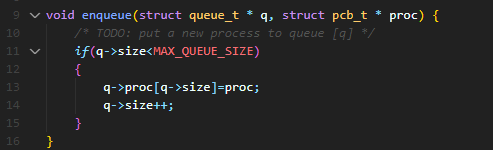
\includegraphics[width=10cm]{enqueue.png}
								\caption{\textit{enqueue() implementation}}
							\end{center}
						\end{figure}
					\item \textit{dequeue()}: Retrieve process with highest priority in queue, update queue status when retrieving element.
						\begin{figure}[h!]
							\begin{center}
								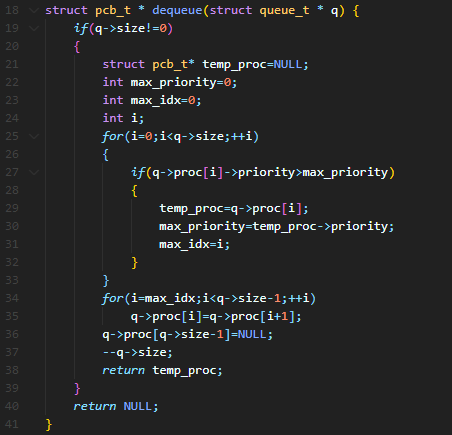
\includegraphics[width=10cm]{dequeue.png}
								\caption{\textit{dequeue() implementation}}
							\end{center}
						\end{figure}
				\end{enumerate}
			\newpage
			\subsubsection{Scheduler}
				The scheduler is used to manage updating the processes that will be executed for the CPU. \\
				We use \textit{get$\_$proc()} in \textit{sched.c} to implement scheduler in this project.\\
				\textit{get$\_$proc()} will return the process at queue ``ready''. If queue is empty at the time function is called, update queue again with processes that are waiting for next slot in queue ``run''. On the contrary, we find the process with high priority from this queue.
				\begin{figure}[h!]
				
	\begin{center}
				
		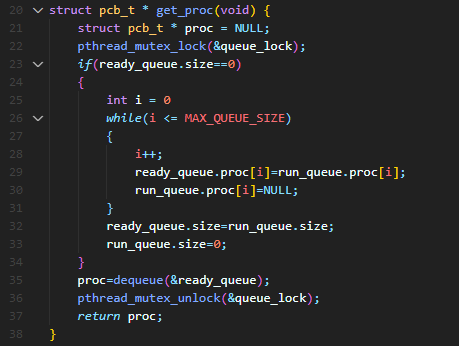
\includegraphics[width=7cm]{get_proc.png}
				
		\caption{\textit{get$\_$proc() implementation}}
				
	\end{center}
				\end{figure}
			\newpage
			
			After run command \textit{make test$\_$sched} by terminal, we can see result like this:
			\begin{figure}[h!]
				\begin{center}
					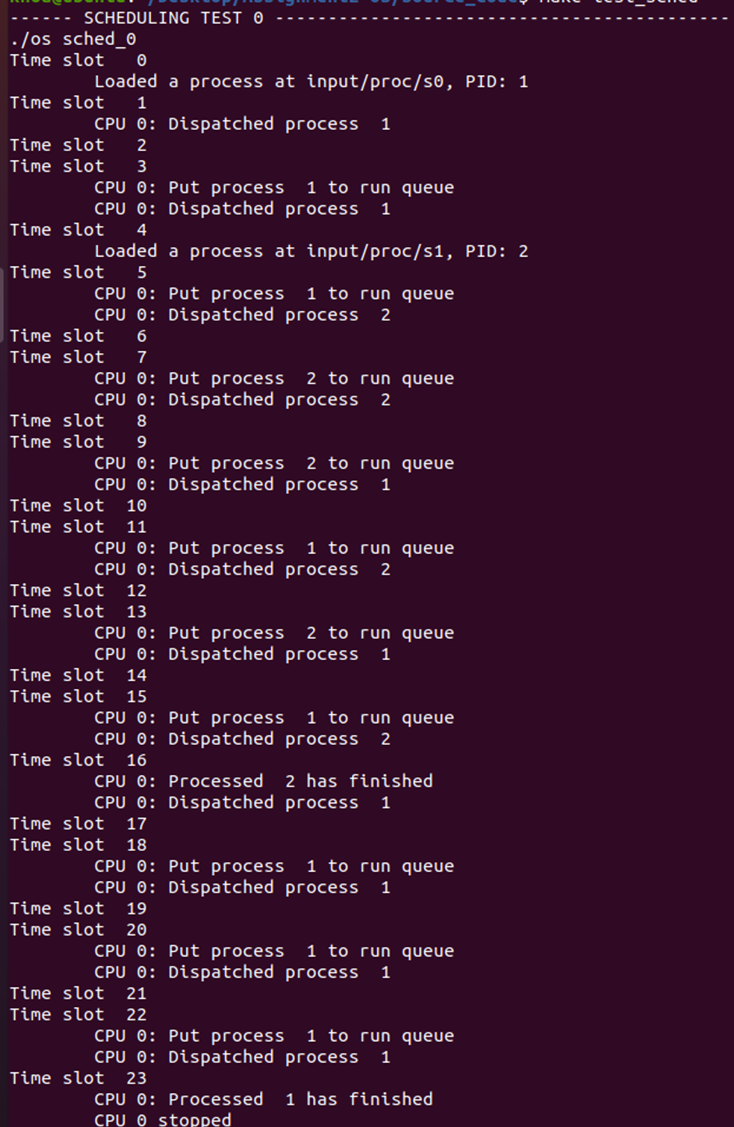
\includegraphics[width=7cm]{test_sched_1.png}
					\caption{\textit{Scheduling Test 1 result}}
				\end{center}
			\end{figure}
			\newpage
			\begin{figure}[h!]
				\begin{center}
					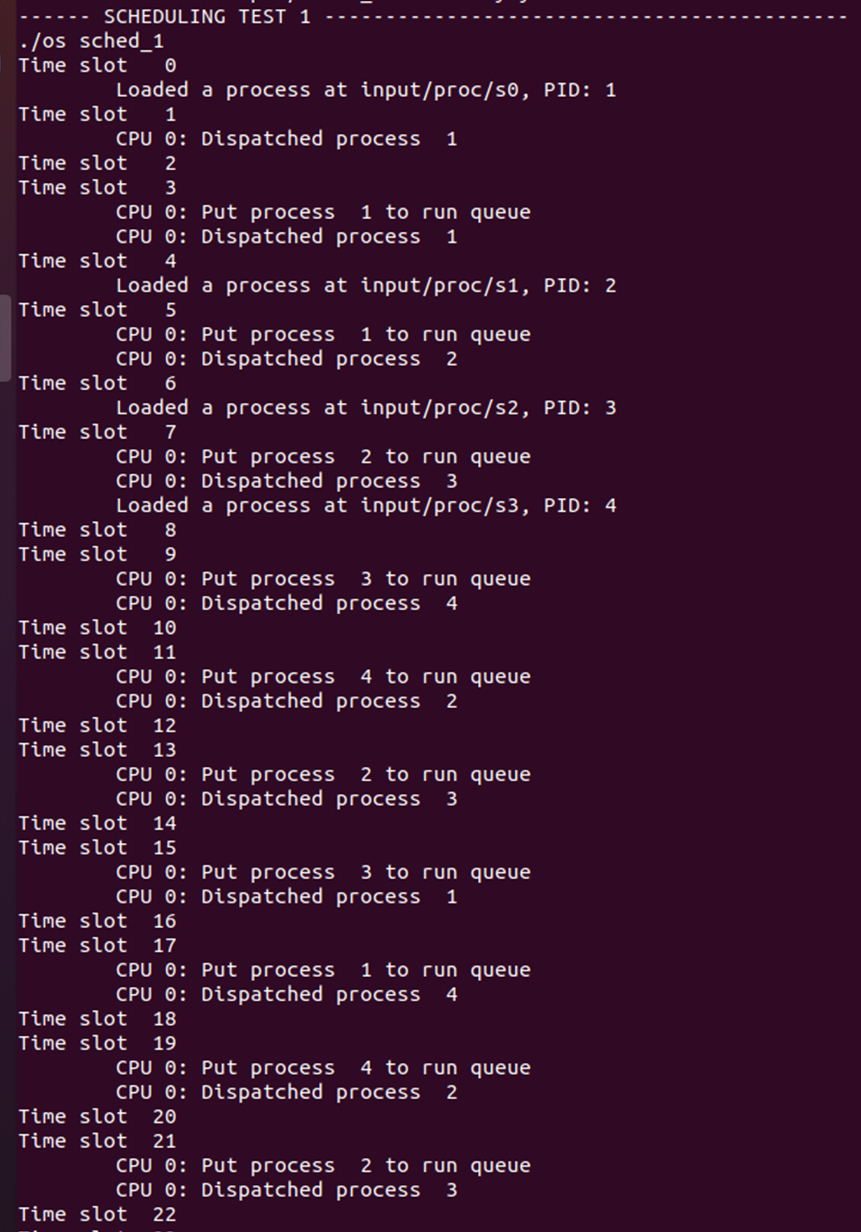
\includegraphics[width=7cm]{test_sched_2_1.png}
					\caption{\textit{Scheduling Test 2 result (1)}}
				\end{center}
			\end{figure}
			\begin{figure}[h!]
				\begin{center}
					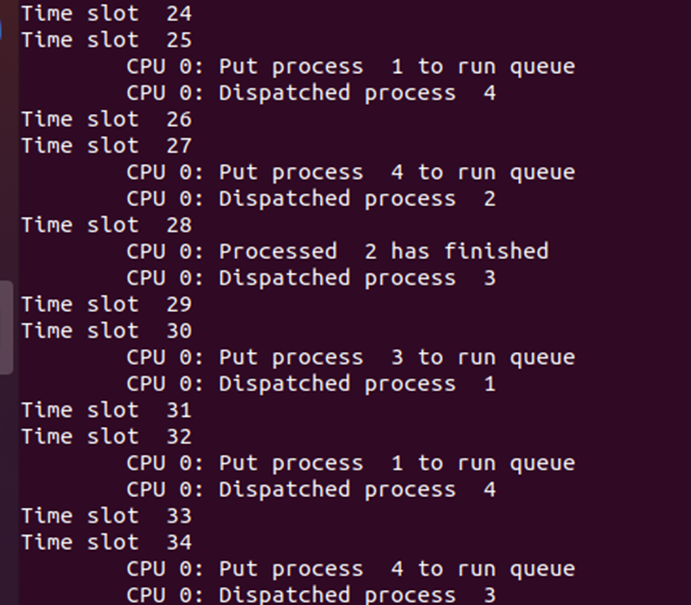
\includegraphics[width=7cm]{test_sched_2_2.png}
					\caption{\textit{Scheduling Test 2 result (2)}}
				\end{center}
			\end{figure}
			\newpage
			\begin{figure}[h!]
				\begin{center}
					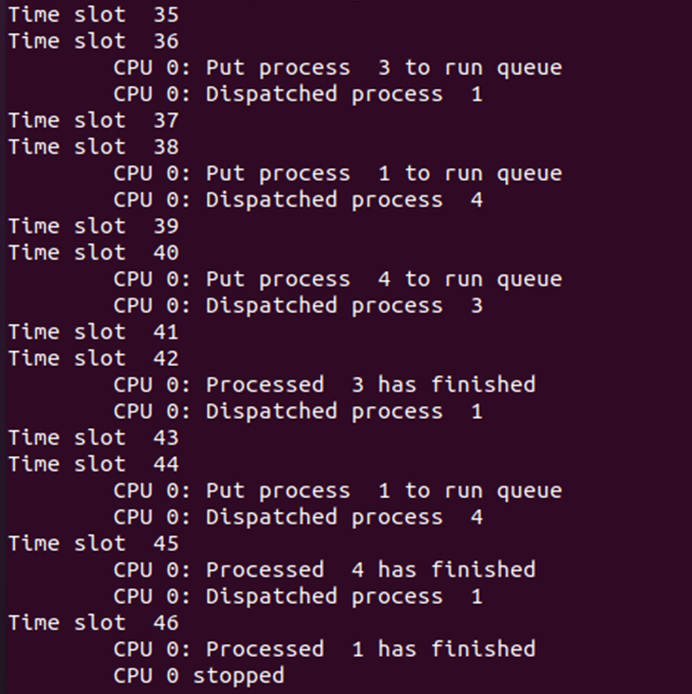
\includegraphics[width=7cm]{test_sched_2_3.png}
					\caption{\textit{Scheduling Test 2 result (3)}}
				\end{center}
			\end{figure}
		\subsection{Gantt Diagrams}
			In this Assignment, my team draw Gantt Diagrams to describe how processes are executed by the CPU in 2 situations.
			\subsubsection{Test 1}
				In this situation, CPU executes 2 processes p1 and p2 in 23 time slots.\\
				Gantt Diagrams:
				\begin{figure}[h!]
					\begin{center}
						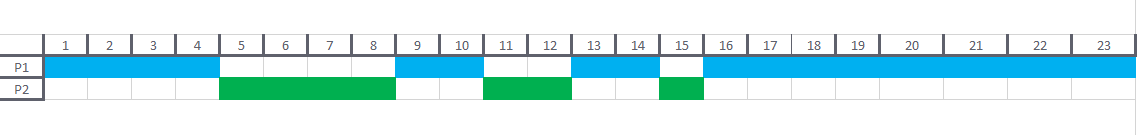
\includegraphics[width=15cm]{gantt_0.png}
						\caption{\textit{Gantt diagram in test 1}}
					\end{center}
				\end{figure}
			\subsubsection{Test 2}
				In this situation, CPU executes 4 processes p1, p2, p3 and p4 in 48 time slots.\\
				Gantt Diagrams:
				\begin{center}
					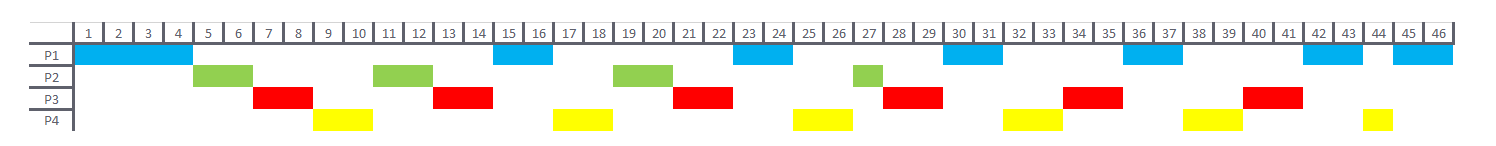
\includegraphics[width=15cm]{gantt_1.png}
				%	\caption{\textit{Gantt diagram in test}}
				\end{center}
	\section{Memory management}
		\subsection{Questions}
			\textbf{Question 2: What is the advantage and disadvantage of segmentation with paging?}\\
			Segmentation with paging is a mechanism Virtual Memory Engine (VME) used to manage memory. \\
			The segmentation technique satisfies the program's need to demonstrate the logical structure of the program, but it leads to the situation of having to allocate memory blocks of different sizes for segments in the physical memory. Therefore, if we do Paging the segmentation, the problem will be better resolved.\\
			Segmentation with paging:
			\begin{enumerate}[-]
				\item Address space is a set of segments, each segment is divided into many pages.
				\item When a process is put into OS, it will allocate to the process necessary pages to contain all segments of the process.
				\item Cuz the process uses virtual addresses to access RAM, we should set the virtual addresses of the allocated pages to be adjacent.
			\end{enumerate}
			Advantage of Segmentation with paging:
			\begin{enumerate}[-]
				\item Saving memory, using memory effectively.
				\item Allocating intermittent memory in a simpler way.
				\item Taking advantages of Paging and Segmentation and minimize disadvantages of each other.
				\item Sharing data between processes is more flexible
				\item Fixing the size of the page too large by paging in each segment.
				\item There is no foreign fragmentation.
			\end{enumerate}
			Disadvantage of Segmentation with paging:
			\begin{enumerate}[-]
				\item Size of the process is limited by the size of physical memory.
				\item It is difficult to maintain multiple processes at the same time in memory.
				\item Page tables need a lot of memory space, so it is not good for systems with small RAM.
			\end{enumerate}
		\subsection{Implement and show the status of RAM}
			We use \textit{alloc$\_$mem()} and \textit{free$\_$mem()} in \textit{mem.c} to implement the status of RAM in this project.\\
			\textit{alloc$\_$mem()}: Allocation memory for the process and save the address of the first byte in the allocated memory region. \newpage
			\begin{figure}[h!]
				\begin{center}
					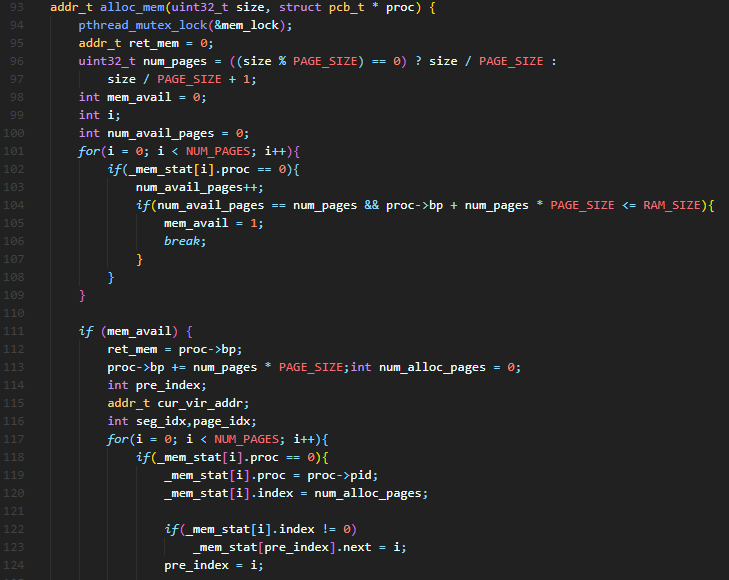
\includegraphics[width=10cm]{allocmem_1.png}
					\caption{\textit{alloc$\_$mem() implementation(1)}}
				\end{center}
			\end{figure}
			\begin{figure}[h!]
				\begin{center}
					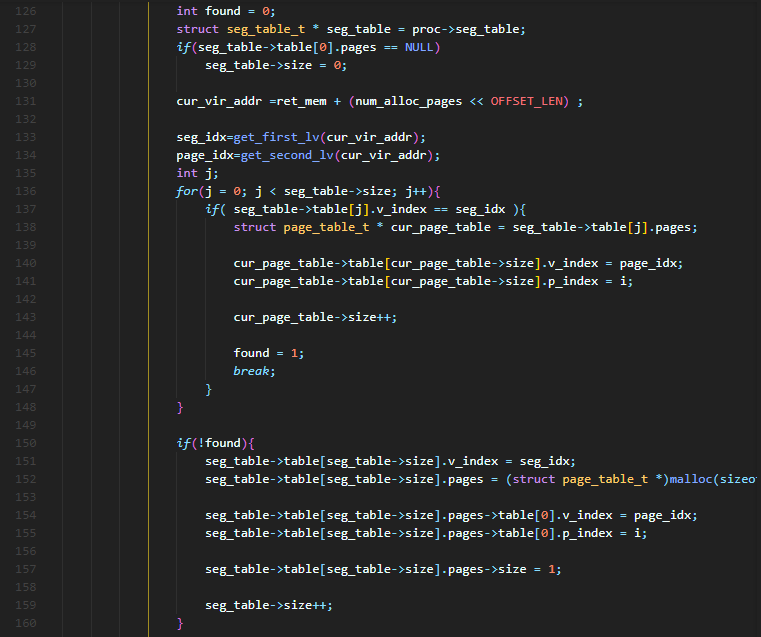
\includegraphics[width=10cm]{allocmem_2.png}
					\caption{\textit{alloc$\_$mem() implementation(2)}}
				\end{center}
			\end{figure}
			\newpage
			\begin{figure}[h!]
				\begin{center}
					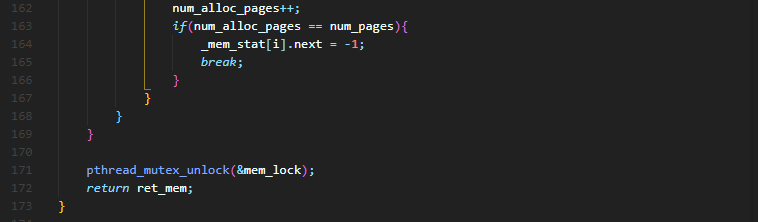
\includegraphics[width=10cm]{allocmem_3.png}
					\caption{\textit{alloc$\_$mem() implementation(3)}}
				\end{center}
			\end{figure} 
			\textit{free$\_$mem()}: Release memory region allocated.
			\begin{figure}[h!]
				\begin{center}
					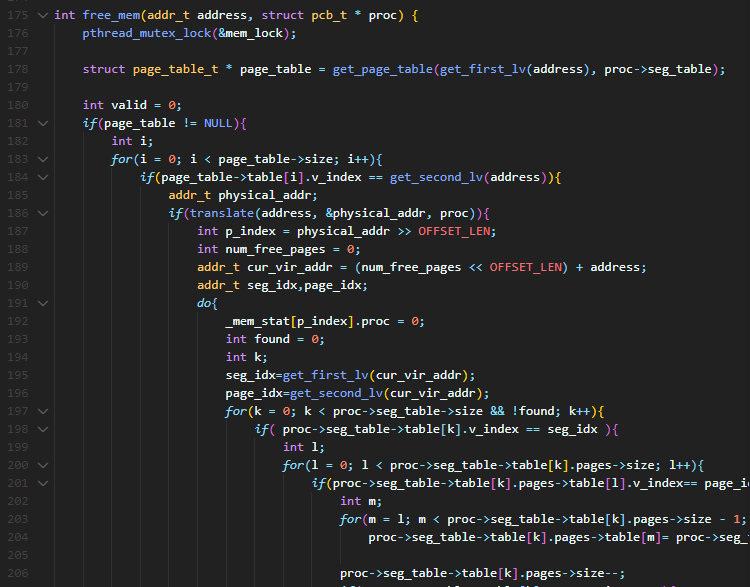
\includegraphics[width=10cm]{freemem_1.png}
					\caption{\textit{free$\_$mem() implementation(1)}}
				\end{center}
			\end{figure}
			\begin{figure}[h!]
				\begin{center}
					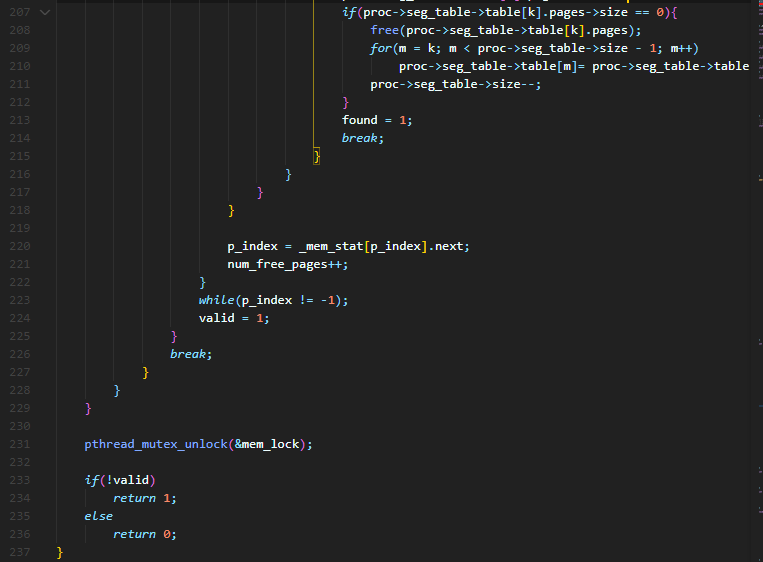
\includegraphics[width=10cm]{freemem_2.png}
					\caption{\textit{free$\_$mem() implementation(2)}}
				\end{center}
			\end{figure}
			\newpage
			After run command \textit{make test$\_$mem} by terminal, we can see result like this:
			\begin{figure}[h!]
				\begin{center}
					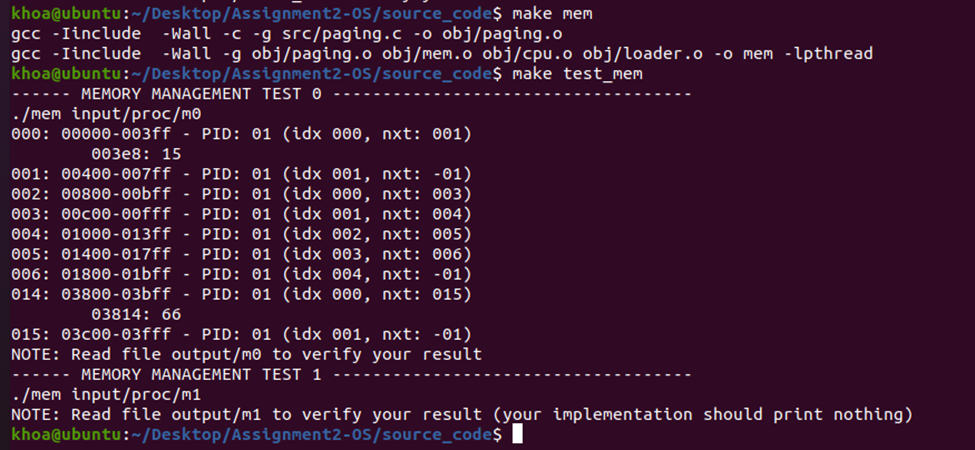
\includegraphics[width=10cm]{testmem.png}
					\caption{\textit{test$\_$mem result}}
				\end{center}
			\end{figure}
		\subsection{Explain file input m0}
				\begin{center}
					\begin{tabular}{lll}
						\hline \\
						1 7 & & \\
						alloc 13535 0 & & \\
						alloc 1568 1 \\
						free 0 \\
						alloc 1386 2 \\
						alloc 4564 4 \\
						write 102 1 20 \\
						write 21 2 1000 \\
						\hline\\
					\end{tabular}
				\end{center}
				\begin{enumerate}[-]
					\item In first line, ``1'' is the priority of process m0, and ``7'' is the instruction number of the input file.
					\item In 2nd line, comment ``alloc 13535'' will allocate 14 $\_$mem$\_$stat pages (from 000 to 013) and store the address of the first allocated byte in register 0.
					\item In 3rd line, comment ``alloc 1568'' will allocate 2 pages (014 and 015) and store the address of the first allocated byte in register number 1.
					\item In 4th line, comment ``free 0'' will release the allocated memory from the alloc command in register number 0, which means there are only pages 014 and 015 at this time.
					\item In 5th line, comment ``alloc 1386'' will allocate 2 pages (000 and 001), then store the address of the first allocated byte in register number 2.
					\item In 6th line, comment ``alloc 4564'' will allocate 5 pages (from 002 to 006) and store the address of the first allocated byte in register number 4.
					\item In 7th line, comment ``write 102 1 20'' will write the value 102 to the place where the address is equal to register address 1 plus an offset of 20 that will output 0x03814.\\ The physical address can be calculated by $ Physical\ address = Base\ address + Offset$, in which, $Base\ address = 0x03800$ is the first byte and $offset = 20$.  
					\item In final line, similarly, the result would be 003e8.
				\end{enumerate}
	\section{Overall}
			In file \textit{mem.c}, in addition to the \textit{alloc$\_$mem()} and \textit{free$\_$mem()}, we also implement \textit{get$\_$page$\_$table()} and \textit{translate()}. Besides, we fixed \textit{read$\_$mem()} and \textit{write$\_$mem()}, too.\newpage
			\textit{get$\_$page$\_$table()} is used to find the paging table from segment: \\
			\begin{figure}[h!]
				\begin{center}
					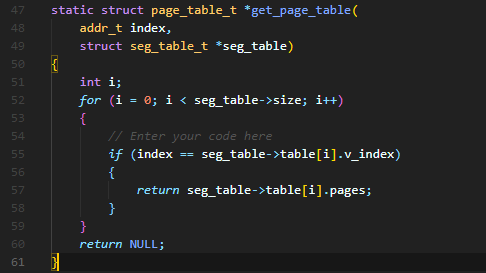
\includegraphics[width=10cm]{get_page.png}
					\caption{\textit{get$\_$page$\_$table() implementation}}
				\end{center}
			\end{figure} \\
			\textit{translate()} is used to map virtual addresses to physical addresses: \\
			\begin{figure}[h!]
				\begin{center}
					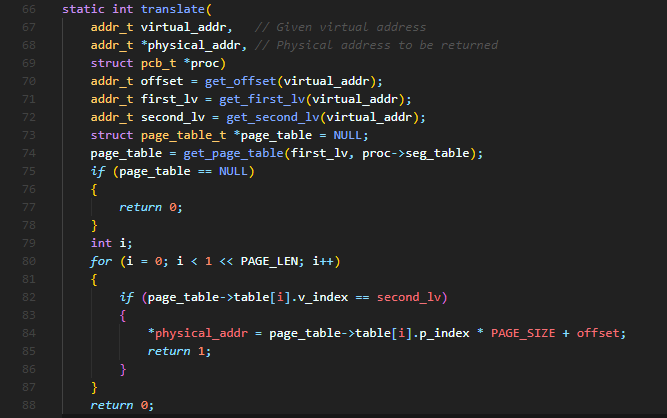
\includegraphics[width=10cm]{translate.png}
					\caption{\textit{translate() implementation}}
				\end{center}
			\end{figure} \newpage
			\textit{read$\_$mem()} and \textit{write$\_$mem()} is added mutex to avoid asynchronous situation when they access to [ram] at the same time.
			\begin{figure}[h!]
				\begin{center}
					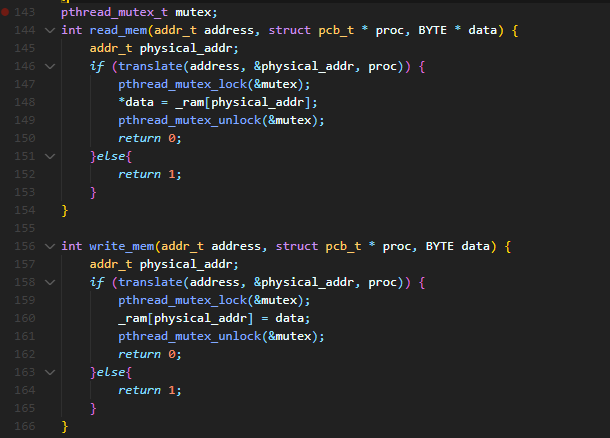
\includegraphics[width=10cm]{mutex.png}
					\caption{\textit{read$\_$mem() and write$\_$mem() after added mutex}}
				\end{center}
			\end{figure}
		\newpage
	\section{Simulation}
		After run command \textit{``make test$\_$all''} by Terminal, we can see result like below:
		\begin{figure}[h!]
			\begin{center}
				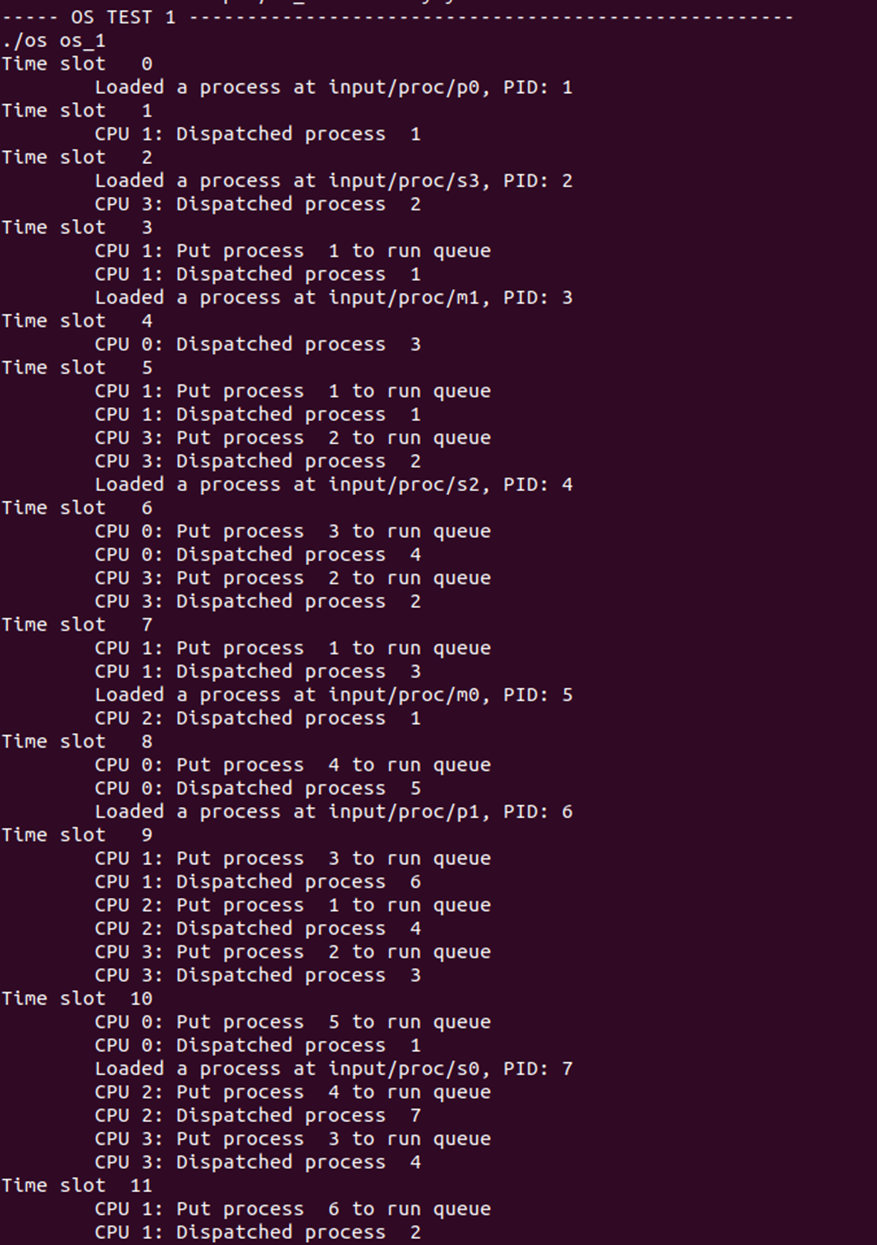
\includegraphics[width=10cm]{final_1.png}
				\caption{\textit{Final result (1)}}
			\end{center}
		\end{figure}
		\begin{figure}[h!]
			\begin{center}
				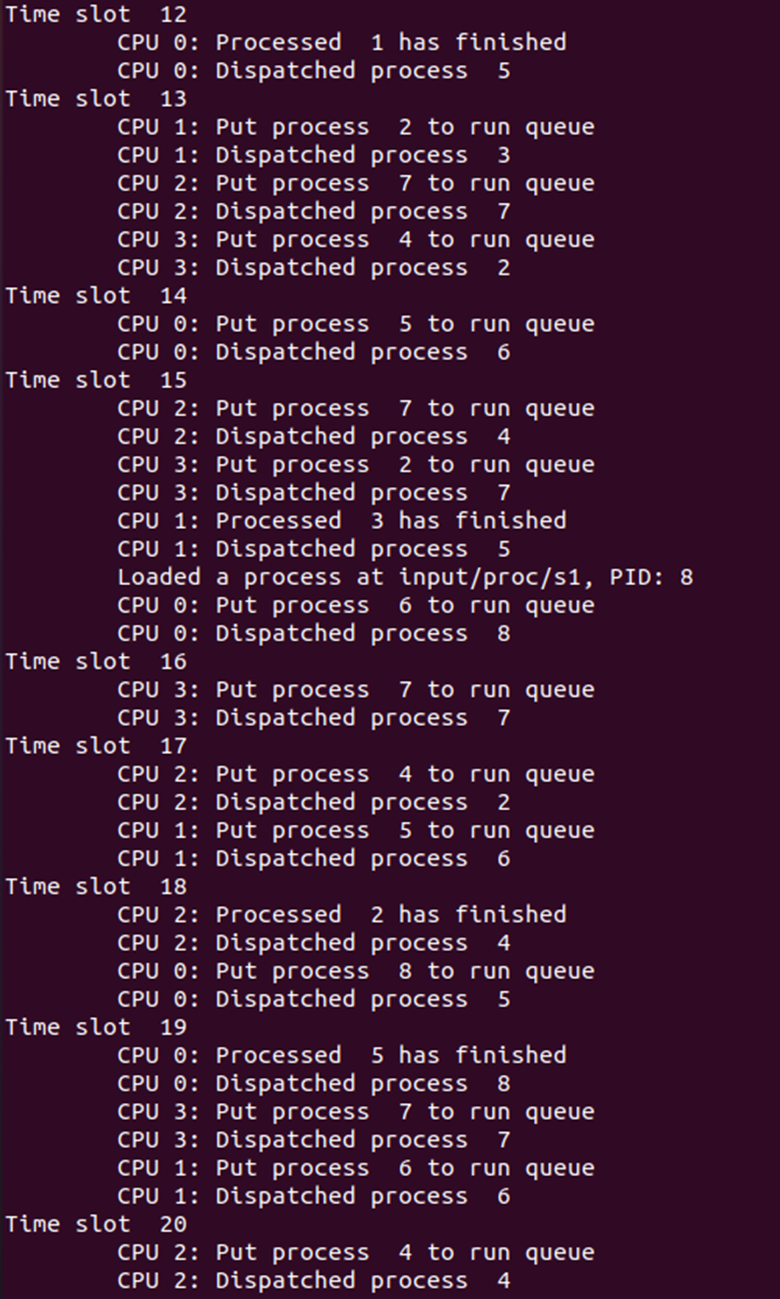
\includegraphics[width=10cm]{final_2.png}
				\caption{\textit{Final result (2)}}
			\end{center}
		\end{figure}
		\begin{figure}[h!]
			\begin{center}
				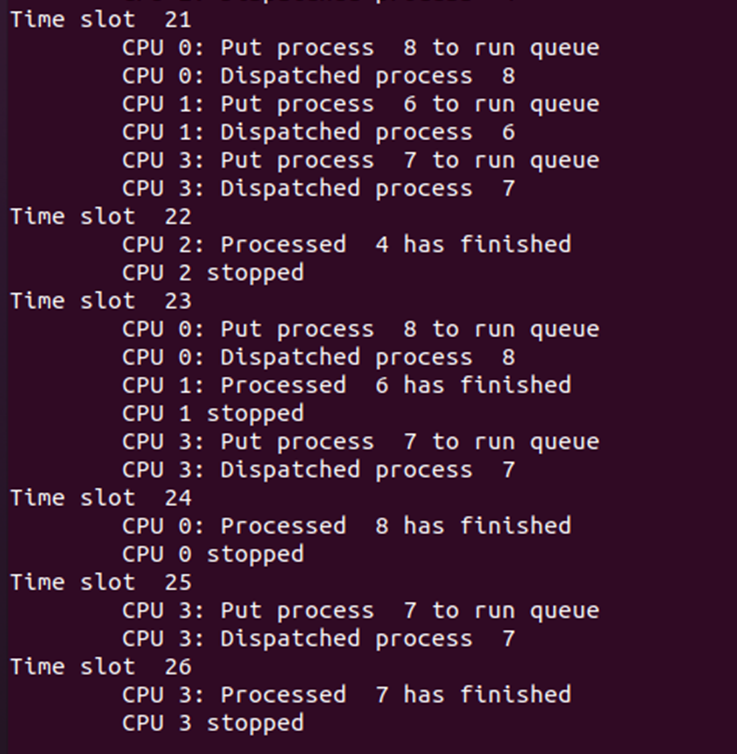
\includegraphics[width=9cm]{final_3.png}
				\caption{\textit{Final result (3)}}
			\end{center}
		\end{figure}
		\begin{figure}[h!]
			\begin{center}
				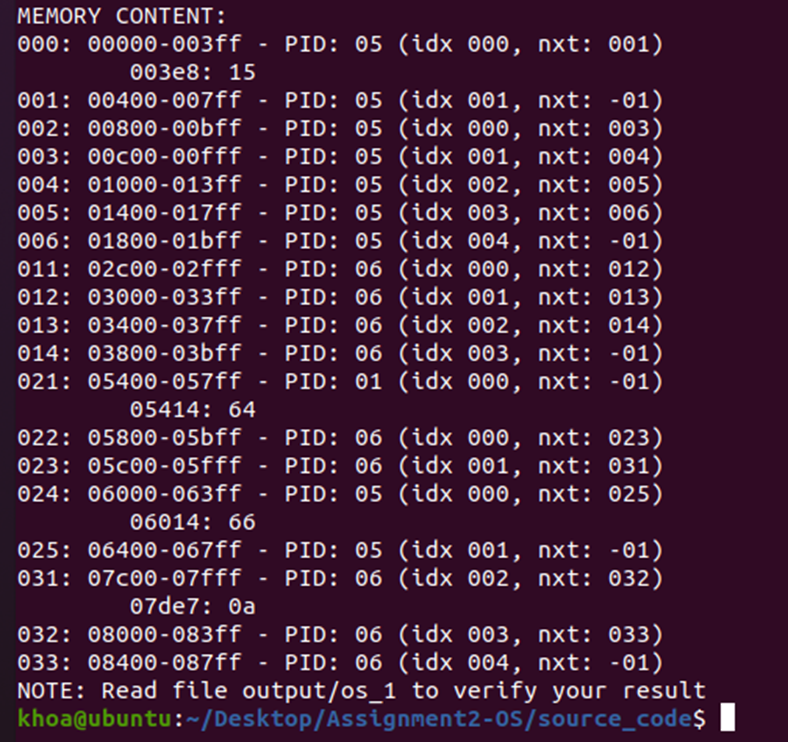
\includegraphics[width=9cm]{final_4.png}
				\caption{\textit{Final result (4)}}
			\end{center}
		\end{figure}
\end{document}